\begin{small}
\begin{verbatim}
% LaTeX (version 2e) source for "LaTeX for Thesis and Large Documents"
% By Stephen Carr and Wail Gueaieb
% Updated 2005-04-07
%
% Parts to edit are marked by the following block:
%###################################
%## Edit this part
%###################################
% 
% Do NOT edit anything else unless you know what you are doing.
%
%======================================================================
%   P R E A M B L E
%======================================================================
\documentclass[%
12pt,   % font size
oneside,  % final version of thesis has to be submitted single-sided
%twoside, % in case you want to print a draft on both sides of the page
]{report} 
%----------------------------------------------------------------------
%###################################
%## Edit this part
%###################################
\newcommand{\thesisauthor}{Stephen M. Carr and Wail Gueaieb}
\newcommand{\thesistitlecoverpage}{%
  \LaTeX \\ 
  for Thesis \\
  and Large Documents
}
\newcommand{\thesistitleheadings}{\LaTeX for Thesis and Large Documents}
\newcommand{\degree}{Ph.D.} % possible values are:
                          % M.A. / M.A.Sc. / M.Sc. / MCS / Ph.D.
\newcommand{\nameofprogram}{Electrical and Computer Engineering}
\newcommand{\academicunit}{School of Information Technology and Engineering}
\newcommand{\faculty}{Faculty of Engineering}
\newcommand{\graduationyear}{2005}

\newcommand{\abstractfile}{abstract.tex}
\newcommand{\acknowledgementfile}{acknowledgement.tex}
%----------------------------------------------------------------------
% Reprocess only those files which have changed recently:
% \includeonly{intro,creating,commands} 
%----------------------------------------------------------------------
% Create a listing in the log of all files needed to process this document
\listfiles
%----------------------------------------------------------------------
\makeindex % activate index-making
%----------------------------------------------------------------------
% THESIS PREAMBLE
% By Stephen Carr and Wail Gueaieb
% Updated 2005-04-07

% The following command sets "1.2" as the line spacing throughout the
% thesis for readability (optional).
\renewcommand{\baselinestretch}{1.2}
%----------------------------------------------------------------------
% Reset page margins properly for doublesided pages
\usepackage[letterpaper,includehead,left=3.25cm,right=2.5cm,top=2.5cm,headsep=1.5cm,headheight=0.0cm,bottom=2.5cm,footskip=1.0cm]{geometry} 
% \setlength{\marginparwidth}{0pt}
% \setlength{\marginparsep}{0pt}
% \setlength{\oddsidemargin}{0.125in}
% \setlength{\evensidemargin}{0.125in}
% \setlength{\textwidth}{6.375in}
\raggedbottom
%----------------------------------------------------------------------
%%%%%%%%%%%%%%%%%%%%%%%%%%%%%%%%%%%%%%%%%%%%%%%%%%%%%%%%%%%%%
 % thesis-specific settings
%----------------------------------------------------------------------
% My own command and environment definitions:
\newcommand{\program}[1]{\textbf{#1}} % program names in bold text
\newcommand{\exten}[1]{\texttt{#1}} % file extensions in bold text (use caps)
\newcommand{\cmmd}[1]{\textbackslash\texttt{#1}} % command name in tt font 
\newcommand{\enviro}[1]{\texttt{#1}} % environment name in tt font

\newcommand{\eg}{\textit{e.g.},} % some Latin abreviations in italic
\newcommand{\ie}{\textit{i.e.},}
\newcommand{\etc}{\textit{etc}.\@}

\newcommand{\mat}[1]{\ensuremath{\mathcal{#1}}} 
	% matrix names in uppercase caligraphic
\newcommand{\vect}[1]{\ensuremath{\mathit{#1}}} 
% vector names in math italic
\newcommand{\rv}[1]{\ensuremath{\mathbf{#1}}} 
% math bold for random variables
\newcommand{\degg}[1]{\mbox{\raisebox{3pt}{$\circ$}\hspace{-.5pt}#1}}
% command to produce a degree sign. Example: \degg[C] gives degrees Celcius

\newenvironment{definition}[1]{\begin{quote}\emph{#1}:}{\end{quote}}
  % Provides indented formal definition and emphasizes the word.
  % e.g. \begin{definition}{Reliability} ... \end{definition}

\newenvironment{where}[1]% Equation symbol lists
 {\begin{list}{}%
  {\renewcommand{\makelabel}[1]{\hfill\textnormal{##1 =}}%
   \settowidth{\labelwidth}{\textnormal{#1 =}}%
   \setlength{\leftmargin}{\labelwidth}%
   \addtolength{\leftmargin}{\labelsep}%
   \setlength{\itemsep}{-\parsep}}}%
 {\end{list}}
% Example:
% \begin{where}{where $E$}
%  \item[where $E$] least squares error term;
%  \item[$w$] weighting factor associated with each measured variable.
% \end{where}
%----------------------------------------------------------------------
% Standard LaTeX2e packages I am using (as seen in "The LaTeX Companion"):
\usepackage[dvips]{graphicx} 
	% ... if you want to include encapsulated postscript figures
\usepackage{makeidx} % ... if you want an index
\usepackage{amsmath} % ... if you need lots of math symbols
\usepackage[dvips=true,bookmarks=true]{hyperref} 
	% ... only needed for PDF generation
%----------------------------------------------------------------------
% Non-standard packages I am using (things I've written, borrowed, etc.):
%\usepackage{} % ... note that old .sty files can be included here

%======================================================================
%   L O G I C A L    D O C U M E N T
%======================================================================
\begin{document}
%----------------------------------------------------------------------
% FRONT MATERIAL
%----------------------------------------------------------------------
% TITLE PAGE 
% By Stephen Carr and Wail Gueaieb
% Updated 2005-04-07

\pagestyle{empty} % No headers or page numbers

\begin{center}

\vspace*{1.0cm}
{\bf \LARGE %
  \thesistitlecoverpage}

\vspace*{1.0cm}
\normalsize
by \\
\vspace*{1.0cm}
\Large
\thesisauthor\\
\vspace*{2.0cm}
\normalsize
Thesis submitted to the\\
Faculty of Graduate and Postdoctoral Studies\\
In partial fulfillment of the requirements\\
For the \degree~degree in\\
\nameofprogram\\

\vspace*{2.0cm}
\academicunit\\
\faculty\\
University of Ottawa\\

\vspace*{2.0cm}
\copyright~\thesisauthor, Ottawa, Canada, \graduationyear\\

\end{center}

\newpage
 
%%%%%%%%%%%%%%%%%%%%%%%%%%%%%%%%%%%%%%%%%%%%%%%%%%%%%%%%%%%%%

% PRELIMINARY PAGES
\pagestyle{plain} % No headers, just page numbers
\pagenumbering{roman} % Roman numerals
\setcounter{page}{2}

%----------------------------------------------------------------------
% This page is not needed for the University of Ottawa
% % Declaration Page
% \noindent
% I hereby declare that I am the sole author of this thesis.

% \noindent
% I authorize the University of Ottawa to lend this thesis to other
% institutions or individuals for the purpose of scholarly research.
% \vspace{4cm}

% \noindent
% \thesisauthor

% \vspace{4cm}

% \noindent
% I further authorize the University of Ottawa to reproduce this thesis by
% photocopying or other means, in total or in part, at the request of other
% institutions or individuals for the purpose of scholarly research.
% \vspace{4cm}

% \noindent
% \thesisauthor
% \newpage
%----------------------------------------------------------------------

% Long abstract (manually formatted)
\begin{center}
\Large
\textbf{Abstract}
\end{center}
\input{\abstractfile}
\newpage

% Acknowledgements and/or Dedication Pages
\begin{center}
\Large
\textbf{Acknowledgements}
\end{center}
\input{\acknowledgementfile}
\newpage

% Pages which are generated automatically
\setcounter{page}{6} % Set this counter to get correct page numbers
% Set the table of content depth. %
\setcounter{tocdepth}{2}
\tableofcontents
\listoftables
\listoffigures
\newpage

% Change page numbering back to Arabic numerals
\pagenumbering{arabic}
%%%%%%%%%%%%%%%%%%%%%%%%%%%%%%%%%%%%%%%%%%%%%%%%%%%%%%%%%%%%%
 
% Title page, declaration, borrowers' page, abstract, acknowlegements, 
% dedication, table of contents, list of tables, list of figures

%----------------------------------------------------------------------
% MAIN BODY
%----------------------------------------------------------------------
% HEADINGS 
% By Stephen Carr and Wail Gueaieb
% Updated 2005-04-07


% Put the document title and page numbers in the header
%\pagestyle{headings}
\pagestyle{myheadings} % Put title on left & chapter heading goes on right by default
\markboth{\thesistitleheadings}{% Go to normal sized type
}
 % Specify thesis headings
%----------------------------------------------------------------------
%###################################
%## Edit this part
%###################################
% Chapters 
% Include your "sub" source files here (must have extension .tex)
\chapter{Introduction}
\label{chapter.Introduction}
\markright{Introduction}

%======================================================================
\section{Background}
%======================================================================
Future transport networks are evolving to support the well-known growth of data traffic and the new emerging network requirements such as fast and flexible service provisioning, multiple grades of Quality of Service (QoS), and fast network restoration. Next generation transport networks are also about the convergence of multiple services - examples of which are layer-3 VPNs, layer-2 VPNs, and the newly emerging optical or layer-1 VPNs [XXX] - on to a single unified data communication network.

Another trend in new service offerings is to provide dynamic, on-demand, and multiple classes of services. To maintain the ability to offer multiple classes of services at a lower cost, network providers are now migrating from a static TDM-like service to a dynamic IP-centric service. Today's existing transport networks are integrated in a multilayered architecture consisting of multiple transport technologies such as packet  \gls{MPLS} (Multi Protocol Label Switching), Asynchronous Transfer Mode (ATM), SONET/Synchronous Digital Hierarchy (SDH) and Wavelength Division Multiplex (WDM). There exists a historical lack of coordination among these layers in controlling protection and restoration and multiple services provisioning.

The typical approach to dynamically provisioning connection-services in a multi-layered transport network is to assume the overlay network model. In this model, each layer is treated as 

This is just to demonstrate the usage of references \cite{saad.book} and \cite{saad1.book} and \cite{saad.book} and \cite{knuth.book} and \cite{zhang.article_typical} and \cite{okada.articledualmonths} and \cite{gupta.conf_typical}

a separate entity having its own separate control plane, with lack of ability of one layer to identify or use resources available in other layers. The upper network layer (client) requests transport services from lower network layers (server). Functions such as resource optimization, traffic engineering, and protection and restoration are handled independently by each layer which makes this model fit to best meet the needs of each individual layer for the selected objectives. Mathematically, this model implies an optimal solution is sought in a multi-dimensional space by sequentially searching different dimensions. Consequently, the optimal solution in this case is search-sequence dependant, and not guaranteed to be a global optimum.
In addition to being vertically multilayered, in many instances in practice, optical transport networks are divided into separate multiple horizontal regions (also known as domains) that have separate management/ownership. In this case, a horizontal hierarchical representation of network topology can be applied to achieve better scalability. Paths that traverse multiple horizontal regions are connected by domain gateways. The gateway, in this case, is a node that either directly connects adjacent network regions- and be jointly owned by the regions it connects- or use inter-region links to connect to other gateways in adjacent network regions.
Independently from the inter-connection model, some IP-based control protocol is required to support automated provisioning of multilayered connections in the network. The main mechanisms needed to guarantee correct operations in a multilayered network are the following: (i) neighbor discovery, (ii) link state update, (iii) route computation, and (iv) path establishment. For example, once a route is computed according to some routing approach, a signaling protocol is invoked to setup and manage the connection. Generalized Multi-Protocol Label Switching (G-MPLS) is emerging as the control-plane solution for such an IP-centric network architecture. A typical GMPLS Next Generation Network (NGN) structure is shown in Figure~\ref{NetworkModelNGN}.

\begin{figure}[t]
\begin{center}
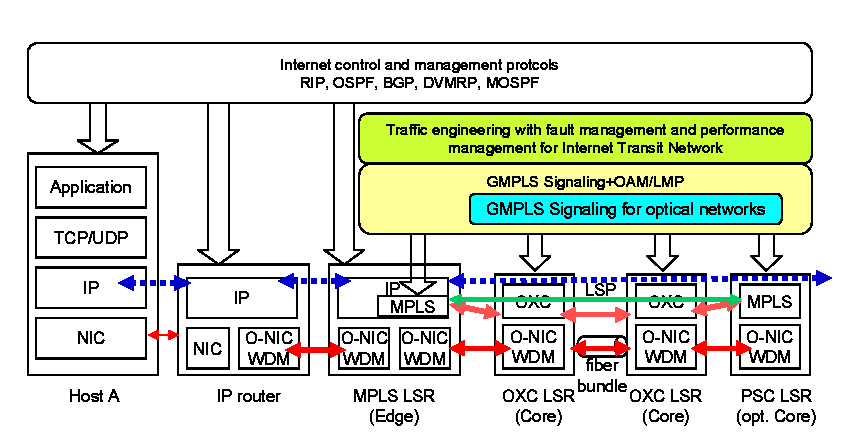
\includegraphics{Figures/NetworkModelNGN} 
\end{center}
\caption{Internet multi-layered traffic engineering model}
\label{NetworkModelNGN}
\end{figure}

Within the context of GMPLS, three basic control plane architectural models have been proposed: the overlay, peer, and the border models. In the peer model, all nodes keep network state information about all links (physical and logical) across all layers of the network. This entails a significant number of control messages to be frequently flooded across network layers to refresh network state information. The overlay model, however, offers total separation between the network switching layers.  The control planes at each of the switching layers operate independently with no exchange of network resource information between adjacent layers. This results in the entire network being managed inefficiently due to the lack of exchanged information. The border model constitutes a compromise between the two previous models where partial network information is exchanged between adjacent layers providing to more efficient and intelligent usage of resources.

Although it is considered that suitable border model architecture can benefit from the advantages of both the overlay and peer models, to our knowledge, there has been a modest effort done to propose efficient provisioning algorithms for this model. As well, within this context, there is little understanding regarding what kind of information would be most helpful in managing routing and signaling decisions in this architecture.

%======================================================================
\section{Motivation}
%======================================================================
Computer networks today have become ubiquitous with increasingly number of services being offered to their end-users. Service Providers (SPs) or network operators are faced with the challenge to support a variety of reliable, secure, and flexible network services and applications to their end-users on a common network infrastructure.
The design configuration, reliability and protection issues of Wavelength Division Multiplexing (WDM) networks have extensively been covered in the literature [GHA00][RIC02] [PHI02][QIN03]. However, most existing networks are integrated in a multiple layer network architecture based on a combination of transport technologies or switching layers where end-to-end connections are likely to span multiple carrier networks. Actually, this multiple layer architecture makes today's core network architecture ineffective. The IP directly over WDM proposition is promising to eliminate unnecessary network layers leading to a reduction in network cost and complexity. However, the challenge remains to control, manage and operate existing transport network effectively using a unified control plane that supports the routing of service requests through a series of regions using dissimilar convergence layers.

A key issue in achieving the above is for the control plane to have knowledge of the multi-layer structure of the network, and how services requested are accommodated. Hence, the coordination, integration and inter-working aspects between the separate network switching layers, on one hand, and the different administrative region-networks, on the other, becomes crucial to facilitate the dynamic provisioning of end-to-end guaranteed services onto a single unified network infrastructure.

When considering optimization of network resources, mathematically, this model implies an optimal solution is sought in a multi-dimensional space by sequentially searching different dimensions-one for each crossed switching layer/domain. Hence, an optimal solution in this case is search-sequence dependant, and not guaranteed a global optimum.

The evolution and maturity of  \gls{MPLS} and Generalized MPLS (GMPLS) has enabled the planning and enabling of advanced networks and services by providers worldwide. GMPLS is a versatile solution addressing current problems at the network level such as scalability, quality of service, traffic engineering, and fast recovery by means of local protection techniques such as Fast Reroute or end-to-end protection schemes [LAN05] [BER05]. GMPLS's unified control plane enables sharing topology and resource information (bandwidth usages, link conditions) across multiple layers. The visibility, however, needs to be carefully controlled in order to meet scalability requirements. One way to achieve this is by aggregating information about resources at lower layers, and presenting the aggregate information to the upper layers. This also eases the integrated design of survivable networks and promises an efficient and cost-effective way to dynamically provisioning multi-grade guaranteed services over a single shared multilayered network, key ingredients of which are bandwidth, latency, service resiliency, and pricing. Active discussions are currently held in IETF working groups [IETFcc], and OIF forums [OIF20] to define metrics and parameters that are required for the routing and signaling in such networks.

Constraint-based path computation is a fundamental building block for traffic engineering in  \gls{MPLS} and GMPLS networks. Specifically, path computation in large, multi-domain, multi-region or multi-layers networks is highly complex and may require special computational 

components and cooperation between the different network domains. A Path Computation Element (PCE) [OKI05] that is present in each node or centralized in each domain is capable of computing optimal and/or diverse TE LSP paths, and providing dynamic inter-layers resource optimization (e.g. optical, and packet layers) of the network's primary and backup capacity. 
In addition, it is imperative to have optimal network resource utilization globally across all network layers to achieve better network efficiency, rather than optimizing resource utilization at each layer independently. This process mandates mechanisms to compute end-to-end paths across layers (inter-layer path computation), and mechanisms for control and management of the virtual network topology (VNT) by setting up and releasing LSPs (or diverse LSPs) in the lower layers.

Approaches to provisioning constrained-based paths are broadly classified into three categories: source routing, distributed hop-by-hop routing, and hierarchical source routing. The hierarchical source routing scheme has been regarded as the most promising scalable approach. However, there is little research on the integration of the hierarchical QoS routing scheme in a GMPLS multilayered network. Additionally, there has been little research investigating mechanisms for supporting QoS/SRLG aggregation schemes suitable in large scale GMPLS networks.
In this context, a multi-grade service offers the benefits of flexibility in service offerings, efficiency in using idle resources, graded pricing to accommodate a wide-spectrum of customers, and the ease of network convergence.

%======================================================================
\section{Objectives}
%======================================================================
The proposed thesis addresses the above raised issues, and presents design constructs and algorithms that suitable for large scale hierarchical layered networks. At present, some of the mathematical analysis and results are at a conjectural stage, the resolutions of which will complete this thesis.

In particular, our objective is to design a multi-layered traffic engineering system that is able to dynamically react to traffic changes while at the same time fulfilling QoS requirements for different classes of service. The main building blocks and operations of the system are:

\begin{itemize}
\item A  \emph{hierarchical aggregation} scheme suitable for the integration in the border model multilayered network architecture. The scheme will be applicable to horizontal as well as vertical layers of the network hierarchy and capable of relaying SRLG and QoS detailed/summarized information for failure-disjoint path calculations.

\item A novel \emph{intelligent path calculation scheme}, within a Path Computation Element (PCE) approach, for the computation of service-constrained optimal and failure diverse LSPs across multiple switching layers and domains. Within this context, two path calculation scheme variants will be considered

\begin{itemize}
\item	scheme that assumes partial/aggregated information about neighboring vertical/horizontal layers. This scheme fits well within a single carrier network managed by a single administrative authority, and

\item a scheme that assumes no/minimal exchange of network state information between layers. 
\end{itemize}
\end{itemize}

In achieving the above, the following is the roadmap sought in the thesis to verify the efficacy of the proposed solutions:

\begin{itemize}
\item Study, design and formulate an analytical mathematical model for multilayer network architecture and apply optimization techniques including Linear Programming and heuristics to achieve network resource utilization optimization.

\item Design dynamic QoS hierarchical routing algorithms suitable for large scale networks, and propose a heuristic for routing QoS/SRLG constrained LSPs

\item Analyze and compare results (e.g. call blocking ratio, crankback frequency, etc.) from simulations run over a hypothetical multi-domain network against optimal solutions achieved using analytical analysis.

\end{itemize}

%======================================================================
\section{Thesis Outline}
%======================================================================
The remainder of this thesis is organized as follows. Chapter 2 describes the hierarchical state of transport networks and the different architectural models that are implemented by network operators today. It also describes interactions between the different switching layers to achieve multi-grade services including multilayered traffic engineering and virtual private networks in the context of GMPLS network architecture. Chapter 3 presents an overview of hierarchical network survivability, and taxonomy of protection and restoration techniques including path diversity across vertical and horizontal layers of the network structure. Chapter 4 presents an overview of network resource aggregation techniques found in the literature and an overview of the related work accomplished in this area, including a novel technique to aggregate for SRLG and QoS resource on links found at different network switching layers, and heuristic algorithm for finding a pair of failure-disjoint working and protection paths. Finally Chapter 5 concludes this report with an identification of work items yet to be finished and a research plan.
 %"What is LaTeX, Why Use It, and Where to Find It?"
\include{chapter2-creating} %"Creating Your Source File"
\include{chapter3-commands} %"Example \LaTeX\ Commands for Large Documents" 
\include{chapter4-processing} %"Processing the Source File"
%----------------------------------------------------------------------
% END MATERIAL
%----------------------------------------------------------------------
%###################################
%## Edit this part
%###################################
% Appendices
\appendix
% Designate with \appendix declaration which just changes numbering style 
% from here on
%\include{useful_pkgs} %"Some Useful \LaTeX2e Packages"
% An appendix
%======================================================================
\chapter{Sources of Information and Help}
\markright{Sources of Information and Help}
%======================================================================
The best source of information about \LaTeX\ is the two books mentioned in this course \cite{lamport.book,goossens.book}.
Another excellent resource is the UseNet newsgroup \verb=comp.text.tex=.
A frequently-asked-questions (FAQ) list is also maintained by this news group.
You might also search the World Wide Web for ``LaTeX'' for other sources of help.
 %"Sources of Information and Help"

% Glossary
% You could use a \begin{description} ... \end{description} for this
\printglossaries 
\newglossaryentry{matrix}{name=Matrix, description=rectangular array of quantities, text=matrix, plural=matrices} 
\newglossaryentry{elite}{name={{�}lite}, description={select group or class}} 
\newglossaryentry{MPLS}{name=MPLS, description=Multiprotol Label Switching}
\newglossaryentry{LSP}{name=LSP, description=Label Switched Path} 
\newglossaryentry{GMPLS}{name=GMPLS, description=Generalized Multiprotol Label Switching}
\newglossaryentry{TE}{name={TE}, description={Traffic Engineering}}
\newglossaryentry{WDM}{name={WDM}, description={Wavelength Division Multiplexing}}
\newglossaryentry{DWDM}{name={DWDM}, description={Dense Wavelength Division Multiplexing}}
\newglossaryentry{VPN}{name={VPN}, description={Virtual Private Network}}
\newglossaryentry{AS}{name={AS}, description={Autonomous System}}
\newglossaryentry{VLAN}{name={VLAN}, description={Virtual Local Area Network}}
\newglossaryentry{SVLAN}{name={SVLAN}, description={Stacked Virtual Local Area Network}}
\newglossaryentry{ISP}{name={ISP}, description={Internet Service Provider}}
\newglossaryentry{SP}{name={SP}, description={Service Provider}}
\newglossaryentry{CSPF}{name={CSPF}, description={Constraint Shortest Path}}
\newglossaryentry{QoS}{name={QoS}, description={Quality of Service}}
\newglossaryentry{SLA}{name={SLA}, description={Service Level Agreement}}
\newglossaryentry{Diffserv}{name={Diffserv}, description={Differentiated Services}}
\newglossaryentry{TDM}{name={TDM}, description={Time Division Multiplexing}}
\newglossaryentry{PSC}{name={PSC}, description={Packet Switching Capable}}
\newglossaryentry{FSC}{name={FSC}, description={Fiber Switching Capable}}
\newglossaryentry{LSC}{name={LSC}, description={Lambda Switching Capable}}
\newglossaryentry{OXC}{name={OXC}, description={Optical Cross Connect}}
\newglossaryentry{RWA}{name={RWA}, description={Routing and Wavelength Assignment}}
\newglossaryentry{DS-TE}{name={DS-TE}, description={Differentiated Services Traffic Engineering}}
\newglossaryentry{P2MP-TE}{name={P2MP-TE}, description={Point-to-multi-point Traffic Engineering}}
\newglossaryentry{LSR}{name={LSR}, description={Label Switching Router}}
\newglossaryentry{IGP}{name={IGP}, description={Interior Gateway Protocol}}
\newglossaryentry{BGP}{name={BGP}, description={Broder Gateway Protocol}}
\newglossaryentry{SRLG}{name={SRLG}, description={Shared Risk Link Group}}
\newglossaryentry{ABR}{name={ABR}, description={Area Border Router}}
\newglossaryentry{OSPF}{name={OSPF}, description={Open Shortest Path First}}
\newglossaryentry{ISIS}{name={ISIS}, description={Intermediate System-Intermediate System}}
\newglossaryentry{ASBR}{name={ASBR}, description={Autonomous System Border Router}}
\newglossaryentry{ERO}{name={ERO}, description={Explicit Route Object}}
\newglossaryentry{TED}{name={TED}, description={Traffic Engineering Database}}
\newglossaryentry{PCE}{name={PCE}, description={Path Computation Element}}
\newglossaryentry{PCC}{name={PCC}, description={Path Computation Client}}
\newglossaryentry{PCEP}{name={PCEP}, description={Path Computation Engine Protocol}}
\newglossaryentry{BRPC}{name={BRPC}, description={Backward Recursive PCE-based Computation}}
\newglossaryentry{LRT}{name={LRT}, description={Link Resource Tree}}
\newglossaryentry{ALRT}{name={ALRT}, description={Aggregate Link Resource Tree}}


% Bibliography 
% If done using the BibTeX program, use
\bibliographystyle{plain} % sorted alphabetically, labeled with numbers
\bibliography{bibliography/keylatex} % names file keylatex.bib as my bibliography file 
% OR, do it "by hand" inside a "thebibliography" enivironment

% Index 
% Put a \makeindex command in the Preamble if you use MakeIndex program
% and put 
\printindex % here
% OR, do it "by hand" inside \begin{theindex} ... \end{theindex}
%----------------------------------------------------------------------
\end{document}
%======================================================================
\end{verbatim}
\end{small}
